\iffalse
\documentclass[journal,12pt,twocolumn]{IEEEtran}
\usepackage{graphicx}
\usepackage[margin=0.5in]{geometry}
\graphicspath{{./figs/}}{}
\usepackage{amsmath,amssymb,amsfonts,amsthm}
\newcommand{\myvec}[1]{\ensuremath{\begin{pmatrix}#1\end{pmatrix}}}
\usepackage{listings}
\usepackage{watermark}
\usepackage{titlesec}
\let\vec\mathbf
\lstset{
frame=single, 
breaklines=true,
columns=fullflexible
}
%\thiswatermark{\centering \put(0,-105.0){
\includegraphics[scale=0.5]{iith.png}} }

\title{\mytitle}
\title{
Matrix Assignment - Conics
}
\author{Adarsh Kumar (FWC22068)}
\begin{document}
\maketitle
\tableofcontents
\bigskip


\section{\textbf{Problem}}
The Area bounded by the Y-axis,Y = Cos(x) and X = Sin(x),
When $0 \le x \le \pi/2$ is :
\linebreak
A) $2(\sqrt{2}-1)$ \\ B) $\sqrt{2}-1$\\ C) $\sqrt{2}+1$ \\D) $\sqrt{2}$
\\
\section{\textbf{Figure}}
\begin{figure}[h]
    \centering
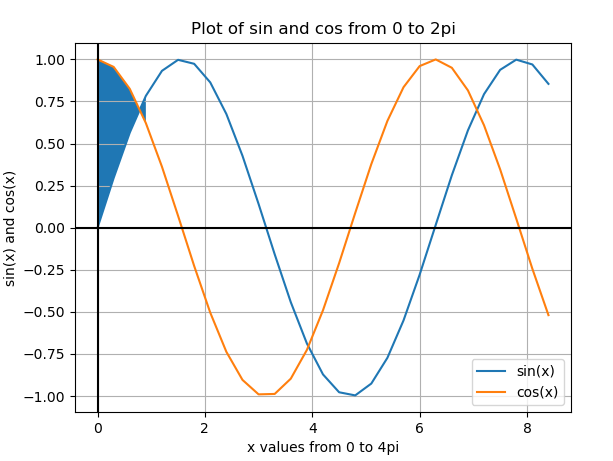
\includegraphics[width=\columnwidth]{conic.png}
    \label{fig:my_label}
\end{figure}
\section{\textbf{Solution}}
As we can see from the figure that , the area bounded by y axis between the limit 0 to $\pi/4$ is only by the positive part of the cosine graph , And that too between 0 to $\pi/4$ .\\
i.e the BLUE shaded region.\\
So, we can further reduce the limits from $ 0 \le x \le \pi/2$ to 
$ 0 \le x \le \pi/4$ .
So Now
The area bounded by the Y - axis in the given problem can be found by :
\begin{align}
A = \int_{0}^{\pi/4} \cos x \,dx -  \int_{0}^{\pi/4} \sin x \,dx 
\end{align}
\\
which can be reduced as : 
\begin{align}
A =\int_{0}^{\pi/4} (\cos x - \sin x) \,dx
\end{align}
\begin{align}
A = (\cos{\pi/4} + \sin{\pi/4}) - (\cos{0} + \sin{0}) 
\end{align}
\begin{align}
A = (\frac{1}{\sqrt{2}}+ \frac{1}{\sqrt{2}}) - (1+0) 
\end{align}
\begin{align}
A = (\frac{2}{\sqrt{2}} - 1)
\end{align}
\begin{align}
A = \sqrt{2} -1
\end{align}
\\
So, the area bounded by Y-axis is $\sqrt{2}-1$ .\\
So, we can conclude that option B is the correct answer.
 


\section{\textbf{Code Link}}

\begin{lstlisting}
https://github.com/aadrshptel/Fwc_module1/tree/main/Assignments/Matrix%20assignments/Conics/codes
\end{lstlisting}
Execute the code by using the command\\
\textbf{python3 circle.py}



\end{document}
\fi
